\documentclass{article}[12 pt]
\usepackage{amssymb}
\usepackage{amsthm}
\usepackage{amsmath}
\usepackage{appendix}
\usepackage{array}
\usepackage{geometry}
\usepackage{enumitem}
\usepackage{graphicx}
\usepackage{subfig}
\usepackage{caption}
\usepackage{url}
\usepackage{float}
\usepackage{pdfpages}
\usepackage{shortvrb}
\usepackage{mathtools}
\usepackage{multirow}
\usepackage{hyperref}
\usepackage{algorithm}
\usepackage[noend]{algpseudocode}
\usepackage{bm}

\def\BibTeX{{\rm B\kern-.05em{\sc i\kern-.025em b}\kern-.08em
		T\kern-.1667em\lower.7ex\hbox{E}\kern-.125emX}}
\graphicspath{{"C:/Users/Conma/Documents/ImageProcessing/HW05/Report/Images/"}}
% \graphicspath{{"//ece-azare-nas1.ad.ufl.edu/ece-azare-nas/Profile/cmccurley/Desktop/ImageProcessing/HW04/Report/Images/"}}
\geometry{margin=1 in}

\newcommand{\smallvskip}{\vspace{5 pt}}
\newcommand{\medvskip}{\vspace{50 pt}}
\newcommand{\bigvskip}{\vspace{100 pt}}
\newcommand{\tR}{\mathtt{R}}

%===================================================================================================================
\begin{document}
	
\begin{center}
	\textbf{\Large Connor McCurley} \\
	EEE 6512 \qquad \textbf{\large Homework 5 Due November 3, 2018} \qquad Fall 2018 
\end{center}

%===================================================================================================================
\section*{Part I MATLAB Programming}

For this question, we were provided the following image (Fig. \ref{scene}) and asked to separate the foreground (lake) from the background (rest of the image). 
\begin{center}
	\begin{figure}[H]
		\centering
		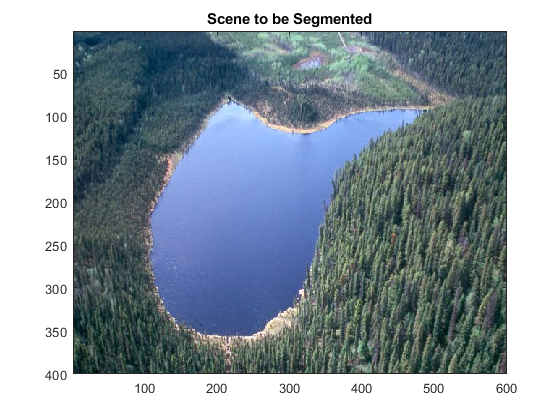
\includegraphics[width = 0.5\textwidth]{Images/scene.png}
		\caption{RGB scene to be segmented}
		\label{scene}
	\end{figure}
\end{center}

\noindent
To accomplish the segmentation, I first applied Gaussian smoothing to each color channel with $\sigma=2$.  This makes sense to do since we don't want to consider all of the high-frequency "noise" scattered throughout the image, such as in the trees.  Since we only cared about the border regions between the foreground and background, I then applied a Sobel edge detector in each color channel to find the first derivative edges.  The histograms for Otsu's method only considered these edge pixels. The results of the edge detection are shown in Fig.\ref{edges}

\begin{figure}[H]
\captionsetup[subfloat]{labelformat=empty}
\centering
\subfloat[]{
  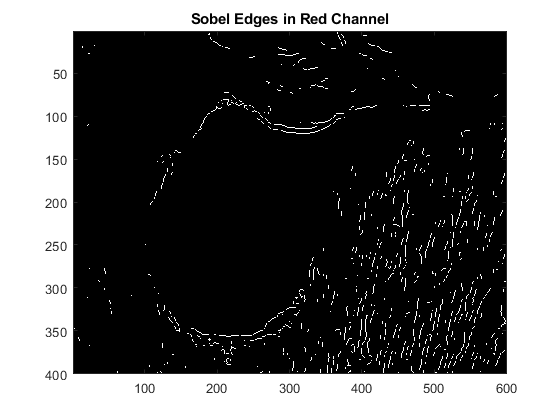
\includegraphics[width=.5\textwidth]{Images/redEdge.png}
} \\
\subfloat[]{
  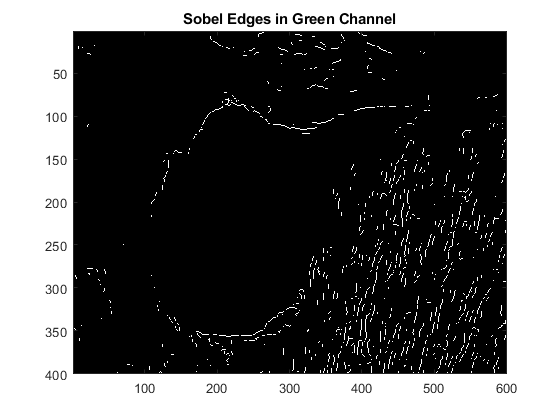
\includegraphics[width=.5\textwidth]{Images/greenEdge.png}
} \\
\subfloat[]{
  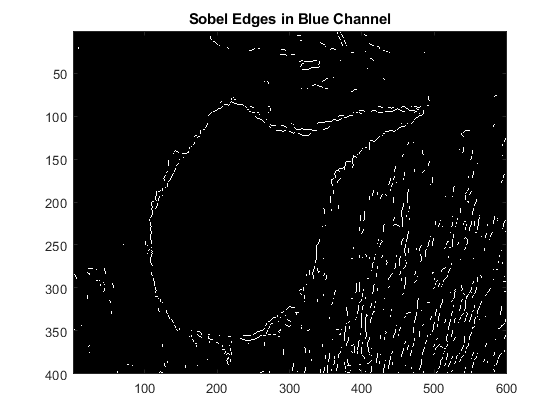
\includegraphics[width=.5\textwidth]{Images/blueEdge.png}
}
\caption{From top to bottom: Sobel edges detected in the red channel, green channel, and blue channel}
\label{edges}
\end{figure}

\noindent
The normalized histogram was found in each color channel using code written for HW02, and only considered the pixels found from the Sobel edge detection.  The normalized histograms of edge pixels are shown in Fig. \ref{hist}.

\begin{figure}[H]
\captionsetup[subfloat]{labelformat=empty}
\centering
\subfloat[]{
  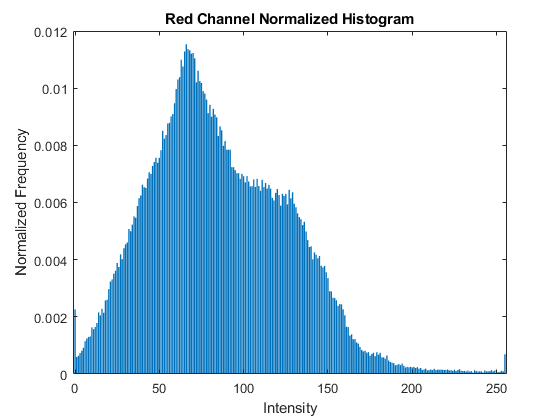
\includegraphics[width=.5\textwidth]{Images/redHist.png}
} \\
\subfloat[]{
  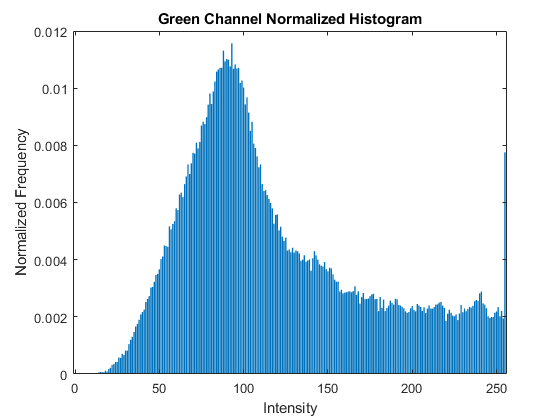
\includegraphics[width=.5\textwidth]{Images/greenHist.png}
} \\
\subfloat[]{
  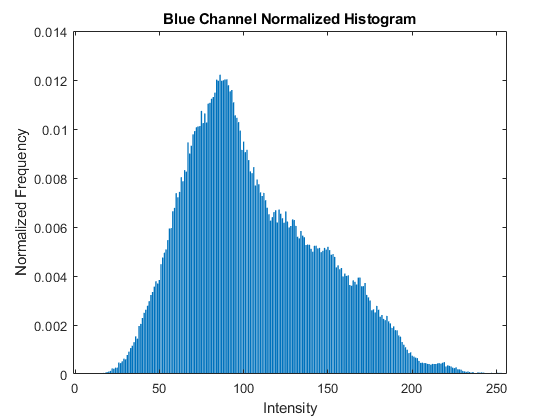
\includegraphics[width=.5\textwidth]{Images/blueHist.png}
}
\caption{From top to bottom: Normalized histogram of Sobel detected edge pixels detected in the red channel, green channel, and blue channel}
\label{hist}
\end{figure}

\noindent
It is clear from the normalized histograms that two modes exist in both the green and blue channels. This was promising for segmentation using Otsu's methods since it effectively finds the optimal boundary between two modes in a distribution. \\

\noindent
Otsu's method was then performed in each color channel following equations 10-49 through 10-62 in the textbook.  The function I wrote, $otsu.m$ took in the rgb scene to be segmented, performed Gaussian filtering, Sobel edge detection, and Otsu's method in each channel.  It then returned a three channel image containing the binary Otsu segmentation for each color channel. The segmentation results using Otsu's Method for each color channel are shown in Fig. \ref{otsu}.

\begin{figure}[H]
\captionsetup[subfloat]{labelformat=empty}
\centering
\subfloat[]{
  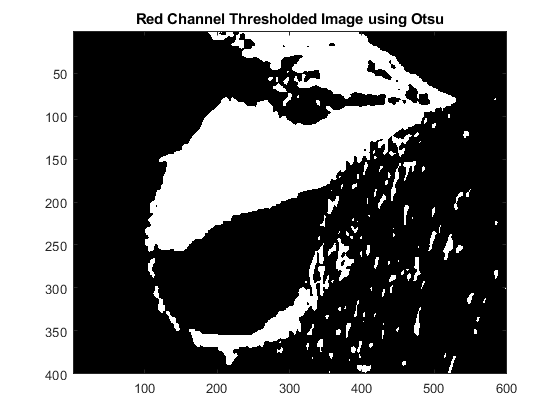
\includegraphics[width=.325\textwidth]{Images/redThresh.png}
} 
\subfloat[]{
  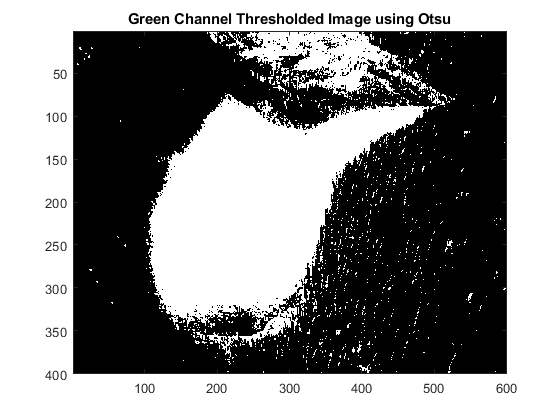
\includegraphics[width=.325\textwidth]{Images/greenThresh.png}
} 
\subfloat[]{
  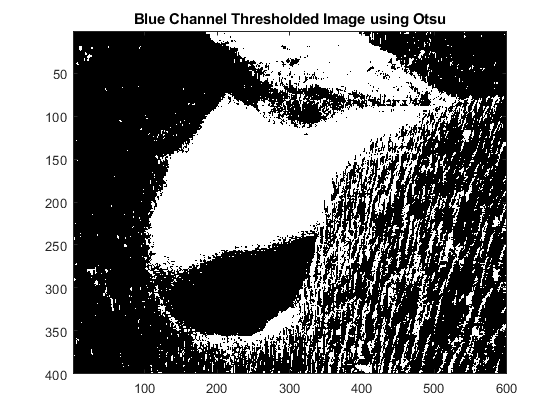
\includegraphics[width=.325\textwidth]{Images/blueThresh.png}
}
\caption{From left to right: Foreground exraction using Otsu's Method in the red channel, green channel, and blue channel}
\label{otsu}
\end{figure}

\noindent
Although it was clear that the blue channel could have been used solely to extract the foreground, we wanted this to be an autonomous process.  Therefore, the channels needed to be aggregated to utilize the foreground information contained in each.  This was accomplished using a logical OR operation between each channel.  The resulting image from  the combination is shown in figure 


\begin{center}
	\begin{figure}[H]
		\centering
		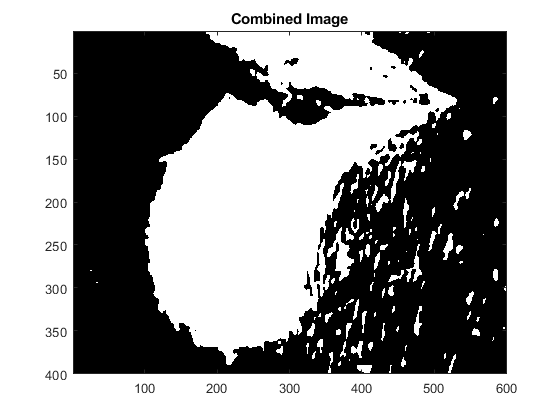
\includegraphics[width = 0.5\textwidth]{Images/combinedImage.png}
		\caption{Binary image formed from the logical OR operation between rgb color channels segmented with Otsu's method}
		\label{scene}
	\end{figure}
\end{center}


\noindent 
The resulting image contained a significant amount of "noise" outside of the foreground.  To remove these spots, morphological opening (erosion then dilation) was utilized to rid the image of spots smaller than a 10x10 disk structuring element (Fig. \ref{openedImage}).

\begin{center}
	\begin{figure}[H]
		\centering
		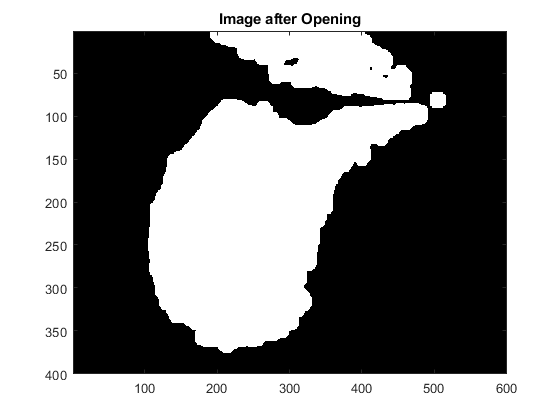
\includegraphics[width = 0.5\textwidth]{Images/openedImage.png}
		\caption{Binary image after opening with a 10x10 disk structuring element}
		\label{openedImage}
	\end{figure}
\end{center}

\noindent
This effectively removed the noisy areas outside of the foreground.  Next, morphological closing (dilation then erosion) with a 15x15 disk structuring element was performed to close the small holes within the foreground (Fig. \ref{closedImage}).  This was necessary before boundary extraction so that no false object boundaries would appear within the foreground.

\begin{center}
	\begin{figure}[H]
		\centering
		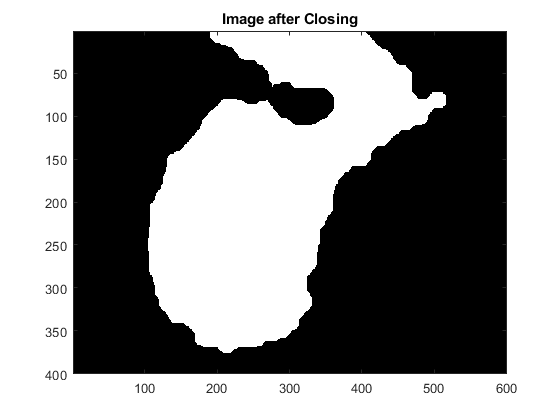
\includegraphics[width = 0.5\textwidth]{Images/closedImage.png}
		\caption{Binary image after closing with a 15x15 disk structuring element}
		\label{closedImage}
	\end{figure}
\end{center}

\noindent
The las step was to extract the boundary of the foreground.  This was done by subtracting the binary image eroded with a 3x3 square of ones structuring element from the binary image.  The eight neighborhood of each pixel on the boundary was set to 1 for visualization.  Results of the boundary extraction are shown in figures \ref{boundMask} and \ref{segmented}.  

\begin{center}
	\begin{figure}[H]
		\centering
		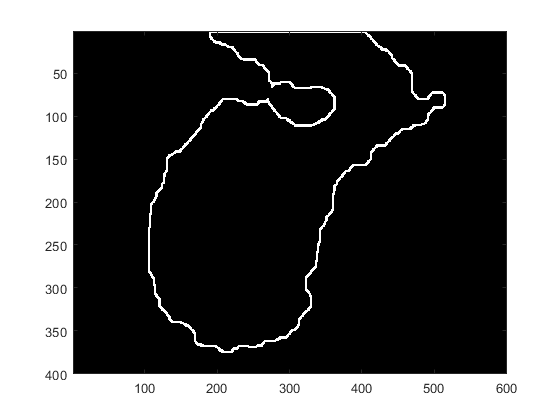
\includegraphics[width = 0.5\textwidth]{Images/boundaryMask.png}
		\caption{Boundary mask found by subtracting the closed image eroded by a 3x3 square of ones from the closed image.  The boundary was widened by setting the eight neighborhood of the boundary pixels to 1's. }
		\label{boundMask}
	\end{figure}
\end{center}
\begin{center}
	\begin{figure}[H]
		\centering
		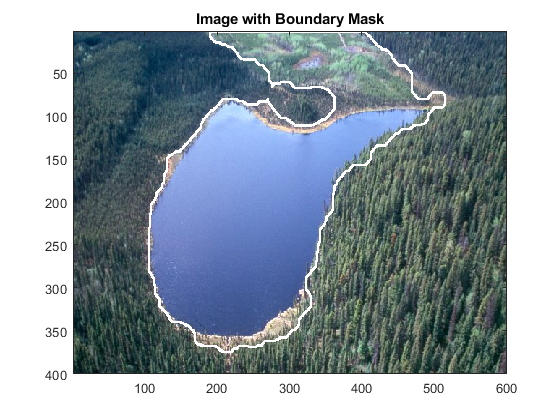
\includegraphics[width = 0.5\textwidth]{Images/segmentedScene.png}
		\caption{Original scene overlain with the computed boundary mask.}
		\label{segmented}
	\end{figure}
\end{center}

\noindent
While segmentation results were not perfect due to many factors such as: smoothing parameters, size and shape of the structuring elements, and the general nature of the image, the entire foreground area was discovered using the selected methods. \\

\noindent
The functions I wrote which were used for this portion of the assignment are as follows:
\begin{enumerate}
\item $mccurleyHW05.m$ - Main function which runs the segmentation.
\item $otsu.m$ - Applies Gaussian filtering, Sobel edge detection, and Otsu's method in each color channel.
\item $extractContours.m$ - Aggregates the three binary images for each channel, performs morphological opening, morphological closing, boundary extraction, and widens the boundary mask.
\item $erodeImage.m$ - Erodes a binary image by a given structuring element.
\item $dilateImage.m$ - Dilates a binary image by a given structuring element. 
\item $plotMask.m$ - Plots the original scene overlain with the computed boundary mask.
\item $myHist.m$ - Computes the normalized histogram of an 8 bit intensity image.
\end{enumerate} 



\section*{Part II Extra Credit}







\end{document}
